\documentclass{article}
\usepackage{listings}
\usepackage{amsmath}
\usepackage{blindtext}
\usepackage{amssymb}
\usepackage{graphicx}
\usepackage[a4paper, margin=1in]{geometry}

\lstset{
	numbers=left,                                        
 	frame=none,                                         
	tabsize=4,
	keywordstyle=\color{blue},
}
\title{Proposal for Master Minds}
\author{Xinhao Su}
\begin{document}
\maketitle
\section{Introduction}
Master Mind is a code breaking game that invented in 1970 by  Mordecai Meirowitz. 
It ressembled from the earlier pencil game 
call Bull and Cows that may date back a century. 
The game play of Master Mind is straight forward:
\begin{enumerate}
	\item The codemaker pick 4 pegs from all the pegs (pegs of 6 different color), and placed them in order as the code. (code can have same color pegs, e.g. red red blue blue)
	\item The codebreaker need to guess both the color and the order of the code within 8 turns. 
	\item At each turn of guess, the codemaker provide feedback by placing 0 to 4 pegs, 
	A black peg indicate that one of the peg in guess is correct in color and order. 
	A white peg indicate that one of the peg in guess is correct in color but not order. 
	\item The game is terminated when codebreaker's guess is correct or all the guesses are incorrect within 8 turns
\end{enumerate}
\begin{figure}[h]
	\centering
	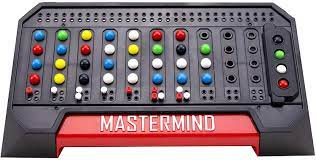
\includegraphics{mm.jpeg}
\end{figure}
Since we will use parallelism to find the solution, our project so called Master Minds


\pagebreak
\section{Algorithm}

The Master Mind game can be rephrase as The Mastermind Problem: 
Given a set of guesses and the number of colored and white pegs scored for each guess, is there at least one secret pattern that generates those exact scores?
The Mastermind Problem has been proved as a NP-Complete problem

\paragraph{Our project will use Five-Guess Algorithm to break the code:}

\begin{enumerate}
	\item Generates set of possible codes, denote as $S$. E.g. $S= \{ 6^4=1296 \ codes\}$
	\item Start with a initial guess, (initial guess can be hardcoded or randomly selected from $S$) 
	\item Play the guess and get response from codemaker
	\item If the program feedback is all black, we found the code.
	\item Otherwise, removed all the codes that would not give the same response in last guess from $S$
	\item Generate next guesses as following:  
\end{enumerate}

\section{Testing Plan}
Since the Mastermind game have many variations, our project intend to test on following variations:
\begin{enumerate}
	\item Mastermind - 6 colors, guessing 4 pegs 
	\item New Mastermind - 8 colors, guessing 4 pegs 
	\item Word Mastermind - 26 letter, guessing 4 letters
	\item Grand Mastermind - 5 colors with 5 shapes, guessing 4 pegs 
	\item Crazy Mastermind - 12 colors, guessing 4 pegs 

\end{enumerate}
\end{document}
